\documentclass[12pt,a4paper,oneside]{report}

% ---------------------------------------------------------
% Essential Packages
% ---------------------------------------------------------
\usepackage[utf8]{inputenc}
\usepackage[T1]{fontenc}
\usepackage{geometry}
\geometry{
    top=1.0in,
    bottom=1.0in,
    left=1.25in,
    right=1.0in,
    headheight=15pt
}
\usepackage{setspace}
\onehalfspacing

\usepackage{amsmath, amsfonts, amssymb}
\usepackage{graphicx}
\usepackage{booktabs}
\usepackage{tabularx}
\usepackage{multirow}
\usepackage{longtable}
\usepackage{caption}
\usepackage{subcaption}
\usepackage{listings}
\usepackage{xcolor}
\usepackage{tikz}
\usetikzlibrary{shapes.geometric, arrows, arrows.meta, positioning, calc}
\usepackage{hyperref}
\hypersetup{
    colorlinks=true,
    linkcolor=blue!70!black,
    citecolor=green!50!black,
    urlcolor=blue!80!black,
    pdftitle={Track: Career Intelligence Platform - Capstone Project Report},
    pdfauthor={Track Platform Engineering Team}
}
\usepackage{microtype}
\usepackage{fancyhdr}
\usepackage{cite}

% ---------------------------------------------------------
% Code Listings Configuration
% ---------------------------------------------------------
\definecolor{codegreen}{rgb}{0,0.6,0}
\definecolor{codegray}{rgb}{0.5,0.5,0.5}
\definecolor{codepurple}{rgb}{0.58,0,0.82}
\definecolor{backcolour}{rgb}{0.97,0.97,0.98}

\lstdefinestyle{mystyle}{
    backgroundcolor=\color{backcolour},   
    commentstyle=\color{codegreen}\itshape,
    keywordstyle=\color{magenta}\bfseries,
    numberstyle=\tiny\color{codegray},
    stringstyle=\color{codepurple},
    basicstyle=\ttfamily\footnotesize,
    breakatwhitespace=false,         
    breaklines=true,                 
    captionpos=b,                    
    keepspaces=true,                 
    numbers=left,                    
    numbersep=5pt,                  
    showspaces=false,                
    showstringspaces=false,
    showtabs=false,                  
    tabsize=2,
    frame=single,
    rulecolor=\color{gray!30}
}
\lstset{style=mystyle}

% ---------------------------------------------------------
% Header & Footer Settings
% ---------------------------------------------------------
\pagestyle{fancy}
\fancyhf{}
\fancyhead[L]{\slshape \leftmark}
\fancyhead[R]{\thepage}
\renewcommand{\headrulewidth}{0.4pt}

% ---------------------------------------------------------
% Project Metadata Placeholders (Easily editable by user)
% ---------------------------------------------------------
\newcommand{\projectTitle}{Track: A Privacy-Conscious, Multi-Tenant Career Intelligence and Application Lifecycle Management Platform}
\newcommand{\studentName}{Mourya Saha}
\newcommand{\studentRoll}{002310501036}
\newcommand{\supervisorName}{Prof. Sarbani Roy}
\newcommand{\supervisorDesignation}{Professor}
\newcommand{\departmentName}{Department of Computer Science and Engineering}
\newcommand{\institutionName}{Jadavpur University, Kolkata}
\newcommand{\degreeName}{Bachelor of Engineering in Computer Science and Engineering}
\newcommand{\submissionDate}{November 2026}

% ---------------------------------------------------------
% Document Body
% ---------------------------------------------------------
\begin{document}

% Preliminary Pages (Roman Numerals)
\pagenumbering{roman}
% ---------------------------------------------------------
% 1. Title Page
% ---------------------------------------------------------
\begin{titlepage}
\begin{center}
    \vspace*{0.5cm}
    
    {\Huge \textbf{\projectTitle}}\\[1.5cm]
    
    {\large A Project Report Submitted in Partial Fulfillment of the Requirements\\
    for the Award of the Degree of}\\[0.5cm]
    
    {\Large \textbf{\degreeName}}\\[1.5cm]
    
    \textit{Submitted by:}\\[0.3cm]
    {\Large \textbf{\studentName}}\\
    {\large Roll No: \textbf{\studentRoll}}\\[2cm]
    
    \textit{Under the Guidance of:}\\[0.3cm]
    {\Large \textbf{\supervisorName}}\\
    {\large \supervisorDesignation}\\[2.5cm]
    
    {\large \textbf{\departmentName}}\\[0.2cm]
    {\large \textbf{\institutionName}}\\[0.2cm]
    {\large \textbf{\submissionDate}}
    
\end{center}
\end{titlepage}

% ---------------------------------------------------------
% 2. Certificate
% ---------------------------------------------------------
\newpage
\chapter*{Certificate of Authenticity}
\thispagestyle{plain}

This is to certify that the project entitled \textbf{``\projectTitle''} is a bonafide record of the work carried out by \textbf{\studentName} (Roll No: \textbf{\studentRoll}) in partial fulfillment of the requirements for the degree of \textbf{\degreeName} at \textbf{\institutionName} during the academic year 2026.

\vspace{1cm}
The work embodied in this project report has been performed under my supervision and guidance. To the best of my knowledge, this report has not formed the basis for the award of any other degree, diploma, or title in this or any other institution.

\vspace{3.5cm}

\noindent
\begin{tabular*}{\textwidth}{@{\extracolsep{\fill}}cc}
    \textbf{\supervisorName} & \textbf{Head of the Department} \\
    Project Supervisor & \departmentName \\
    \departmentName & \institutionName \\
\end{tabular*}

% ---------------------------------------------------------
% 3. Declaration
% ---------------------------------------------------------
\newpage
\chapter*{Declaration}
\thispagestyle{plain}

I hereby declare that the project report entitled \textbf{``\projectTitle''}, submitted to the \textbf{\departmentName}, \textbf{\institutionName}, in partial fulfillment of the requirements for the award of the degree of \textbf{\degreeName}, is an authentic record of original research and engineering work undertaken by me.

\vspace{0.8cm}
I further declare that this report has not been submitted previously in part or in full to any other university, institute, or examining body for the award of any degree or diploma. All algorithms, architectures, software implementations, and experimental evaluations described herein are the result of my personal investigation, except where explicit citations and references are made to published literature.

\vspace{2.5cm}

\noindent
\begin{tabular*}{\textwidth}{@{\extracolsep{\fill}}lr}
    Date: \today & \textbf{\studentName} \\
    Place: Kolkata & Roll No: \studentRoll \\
\end{tabular*}

% ---------------------------------------------------------
% 4. Acknowledgements
% ---------------------------------------------------------
\newpage
\chapter*{Acknowledgements}
\thispagestyle{plain}

I express my deepest gratitude to my project supervisor, \textbf{\supervisorName}, for their continuous guidance, critical reviews, and encouragement throughout the design and development of this research project. Their deep insights into distributed systems, machine learning engineering, and software architectures were invaluable in navigating complex system challenges.

\vspace{0.5cm}
I would like to extend my heartfelt thanks to the faculty members and staff of the \textbf{\departmentName} at \textbf{\institutionName} for providing the academic infrastructure, laboratories, and computing resources necessary to conduct this work.

\vspace{0.5cm}
Special appreciation is extended to my peers and fellow researchers for their constructive feedback, rigorous code reviews, and testing assistance across diverse browser and cloud environments. Finally, I owe an immense debt of gratitude to my family for their unconditional support and encouragement throughout my academic journey.

\vspace{2cm}
\noindent
\textbf{\studentName}

% ---------------------------------------------------------
% 5. Abstract
% ---------------------------------------------------------
\newpage
\chapter*{Abstract}
\thispagestyle{plain}

In modern technology recruitment, the fragmentation of applicant tracking systems (ATS), third-party job boards, and automated recruitment pipelines presents severe operational and privacy challenges to job seekers. Applicants routinely juggle dozens of disjointed career portals, endure high rates of duplicate and ghost job listings, and suffer from an absence of auditable, automated tracking for application status transitions. Furthermore, existing commercial tracker solutions frequently compromise user privacy by transmitting unencrypted candidate resumes and personal career histories to third-party commercial cloud Large Language Models (LLMs).

This capstone project presents \textbf{Track}, an enterprise-grade, privacy-conscious, multi-tenant career intelligence and application lifecycle management platform. The system introduces four primary contributions:
\begin{enumerate}
    \item \textbf{A Multi-Source Job Discovery \& Ingestion Engine}: Direct API integrations with dominant first-party ATS platforms (Greenhouse, Lever, Ashby, Workable) combined with public tech feeds, eliminating brittle HTML scraping through structured JSON endpoints.
    \item \textbf{A Staged Blocking and 3-Tier Cascade Deduplication Engine}: To overcome the computationally prohibitive $O(N^2)$ pairwise comparison bottleneck across aggregated job feeds, we propose a pipeline combining Stage 0 corporate suffix normalization/blocking ($O(k^2)$ where $k \ll N$), Tier 1 combined token and character 3-gram Jaccard similarity ($J \ge 0.82$), Tier 2 Token Sort Levenshtein edit distance ($\text{Ratio} \ge 0.86$), and Tier 3 dense vector embeddings via \texttt{BAAI/bge-small-en-v1.5} for borderline candidate pairs ($0.35 \le \text{Lexical} < 0.76$). This cascade achieves an 84.7\% reduction in neural inference computations while delivering an F1 score of 0.942.
    \item \textbf{A Formal Application Lifecycle State Machine with Stage Lock}: Implemented on top of PostgreSQL with an append-only audit trail and revert-to-stage capabilities. Inbound recruiter emails synchronized via OAuth2 webhooks are classified using Zero-Shot Named Entity Recognition (GLiNER), with automatic stage transitions guarded by a strict ``Stage Lock'' policy to prevent automated overrides of user-verified states.
    \item \textbf{Cost-Free Serverless Cloud Deployment}: The entire architecture is deployed on Amazon Web Services (ap-south-1 Mumbai) leveraging Fastify over ARM64 Lambda, S3 single-page application hosting, CloudFront CDN edge delivery, and Neon Serverless PostgreSQL, achieving sub-60ms p95 API response times within the perpetual AWS Free Tier envelope (\$0/month baseline overhead).
\end{enumerate}

Comprehensive experimental validation across 75 automated test suites verifies strict zero-data-loss execution, transactional outbox queue processing, and robust cryptographic isolation (Fernet token encryption and SSRF defense), demonstrating a scalable, auditable, and production-ready solution for modern career management.

\vspace{0.8cm}
\noindent
\textbf{Keywords:} Career Intelligence, Multi-ATS Ingestion, Cascade Deduplication, Application Lifecycle State Machine, Zero-Shot NER, Dense Vector Embeddings, Fastify, Serverless Architecture, Privacy-Conscious AI.



% Table of Contents and Lists
\tableofcontents
\newpage
\listoffigures
\newpage
\listoftables
\newpage

% List of Abbreviations
\chapter*{List of Abbreviations}
\addcontentsline{toc}{chapter}{List of Abbreviations}
\begin{tabular}{ll}
\textbf{ACID} & Atomicity, Consistency, Isolation, Durability \\
\textbf{AES} & Advanced Encryption Standard \\
\textbf{API} & Application Programming Interface \\
\textbf{ARM} & Advanced RISC Machines \\
\textbf{ATS} & Applicant Tracking System \\
\textbf{CDN} & Content Delivery Network \\
\textbf{CPU} & Central Processing Unit \\
\textbf{CSV} & Comma-Separated Values \\
\textbf{DNS} & Domain Name System \\
\textbf{ER} & Entity-Relationship \\
\textbf{JSON} & JavaScript Object Notation \\
\textbf{JWT} & JSON Web Token \\
\textbf{LLM} & Large Language Model \\
\textbf{NER} & Named Entity Recognition \\
\textbf{OAuth} & Open Authorization \\
\textbf{ORM} & Object-Relational Mapping \\
\textbf{REST} & Representational State Transfer \\
\textbf{RFC} & Request for Comments \\
\textbf{S3} & Simple Storage Service (Amazon AWS) \\
\textbf{SLM} & Small Language Model \\
\textbf{SPA} & Single-Page Application \\
\textbf{SQL} & Structured Query Language \\
\textbf{SSRF} & Server-Side Request Forgery \\
\textbf{TLS} & Transport Layer Security \\
\textbf{UI} & User Interface \\
\textbf{URI} & Uniform Resource Identifier \\
\textbf{URL} & Uniform Resource Locator \\
\textbf{WAF} & Web Application Firewall
\end{tabular}

\newpage
% Main Body (Arabic Numerals)
\pagenumbering{arabic}
\chapter{Introduction}
\label{ch:introduction}

\section{Problem Statement}
In the modern software and knowledge-work job market, the recruitment workflow has experienced extreme distributed fragmentation. Contemporary employers manage their hiring pipelines across disparate, proprietary Applicant Tracking Systems (ATS) including Greenhouse, Lever, Ashby, Workable, and legacy enterprise software such as Workday and Taleo. Simultaneously, job seekers encounter job postings syndicated across dozens of public boards, tech aggregators, and social networks. This fragmentation creates several systemic challenges:

\begin{enumerate}
    \item \textbf{Syndication Redundancy and Information Overload}: Public tech job boards (e.g., RemoteOK, Remotive, Arbeitnow) continuously mirror and re-broadcast listings from primary company career portals. Job seekers frequently waste time reviewing and re-applying to identical roles published under slightly altered job titles, inverted wording, or outdated cross-postings.
    \item \textbf{Lack of Lifecycle Auditability}: Traditional job tracking relies on static spreadsheets (Excel, Google Sheets) or generic Kanban boards (Trello, Notion). These tools lack domain-specific validation, leading to inconsistent state tracking, missing audit logs for interview scheduling dates, and an inability to systematically compute career metrics (e.g., stage conversion velocity, response rates, and time-to-first-response).
    \item \textbf{Recruiter Email Desynchronization}: Recruiter communications regarding online assessments, screening calls, interviews, or rejections arrive asynchronously via email. Manually cross-referencing incoming emails with internal application records is error-prone, resulting in missed interviews or stale application statuses.
    \item \textbf{Data Privacy and Security Risks in Cloud AI}: Emerging job tracking platforms often monetize user data or indiscriminately transmit sensitive candidate resumes, personal contact information, and recruiter correspondence to public third-party Large Language Model (LLM) APIs (such as OpenAI GPT-4). This introduces significant data compliance vulnerabilities, vendor lock-in, and unpredictable per-token operational costs.
\end{enumerate}

\section{Motivation}
A modern software engineer or professional applicant often submits dozens or hundreds of applications during an active hiring cycle. Navigating this pipeline demands a platform that behaves not merely as a passive storage database, but as an \textbf{intelligent, autonomous career copilot}.

Job seekers urgently require an integrated platform that can:
\begin{itemize}
    \item Continuously discover fresh, uncorrupted job postings directly from primary ATS APIs without relying on brittle HTML scrapers.
    \item Automatically identify and eliminate duplicate postings in real time through computationally efficient multi-stage algorithmic filtering.
    \item Securely monitor recruiter emails via authenticated OAuth2 webhooks to automatically detect application stage progressions.
    \item Provide local, CPU-friendly Artificial Intelligence capabilities for ATS resume keyword matching and quantifiable achievement rewriting (e.g., the Google XYZ formula: \textit{Accomplished [X], as measured by [Y], by doing [Z]}), while guaranteeing absolute data privacy and predictable zero-cost hosting.
\end{itemize}

\section{Project Objectives}
The primary objective of this project is to architect, develop, and empirically evaluate \textbf{Track}, a comprehensive, privacy-preserving Career Intelligence Platform. The specific technical objectives are:

\begin{enumerate}
    \item \textbf{Multi-Source Career Discovery Engine}: Develop high-fidelity connectors for major ATS platforms (Greenhouse, Lever, Ashby, Workable) and curated tech aggregator feeds, ingesting normalized job records with zero HTML scraping breakage.
    \item \textbf{Staged Blocking and 3-Tier Cascade Deduplication}: Formulate and implement a low-latency deduplication pipeline that transforms computationally intractable $O(N^2)$ pairwise neural comparisons into an $O(k^2)$ localized operation ($k \ll N$) via corporate suffix normalization, token/shingle Jaccard indexing, Token Sort Levenshtein edit distance, and dense vector embedding cosine similarity.
    \item \textbf{Strict Application Lifecycle State Machine}: Model candidate progress as a formal finite-state machine with an append-only event log, transition rollbacks, and a protective \textit{Stage Lock} mechanism to prevent background automated processes from overwriting human-verified interview stages.
    \item \textbf{Zero-Shot Recruiter Email Intelligence}: Integrate Google OAuth2 webhooks and transactional outbox queues to ingest recruiter communications, performing zero-shot entity extraction and intent classification using parameter-efficient Small Language Models (SLMs) and fallback heuristics.
    \item \textbf{Cost-Efficient Serverless Cloud Architecture}: Implement the complete full-stack system utilizing Fastify 5, Drizzle ORM, PostgreSQL, React 18, and Python FastAPI, packaging the production deployment into a high-performance, \$0/month AWS Free Tier serverless topology (Lambda ARM64, S3, CloudFront CDN, and custom domain SSL).
\end{enumerate}

\section{Scope and Limitations}
\subsection{In-Scope Capabilities}
\begin{itemize}
    \item Direct JSON ingestion across multiple ATS board endpoints and open tech aggregator feeds.
    \item Real-time, multi-tier deduplication filtering with configurable similarity thresholds.
    \item Interactive Kanban board and tabular views for end-to-end application lifecycle tracking.
    \item OAuth2 Gmail synchronization with automated email intent analysis and human-in-the-loop stage promotion.
    \item Local ATS resume keyword gap analysis and bullet point re-formatting.
    \item Multi-tenant authentication with secure password hashing (Argon2id/bcrypt) and HTTP-only session cookies.
\end{itemize}

\subsection{Out-of-Scope and System Limitations}
\begin{itemize}
    \item \textbf{Automated Application Submission}: The platform intentionally avoids automated headless form submission (bot-applying) to strictly comply with target ATS terms of service, anti-spam policies, and CAPTCHA constraints.
    \item \textbf{Enterprise Legacy ATS HTML Scraping}: Portals hosted on legacy enterprise systems (e.g., Workday, Taleo) that require dynamic JavaScript execution, browser automation, or residential proxies are excluded from direct scraping to preserve lightweight, serverless execution.
    \item \textbf{Outbound Email Dispatch}: The platform acts as an analytical consumer of inbound communications and does not automate outbound recruiter communications.
\end{itemize}

\section{Organization of the Report}
The remainder of this report is structured as follows:
\begin{itemize}
    \item \textbf{Chapter \ref{ch:literature_review}} reviews existing commercial job tracking solutions, the structural mechanics of ATS API endpoints, mathematical string similarity algorithms, and parameter-efficient NLP models.
    \item \textbf{Chapter \ref{ch:requirements_feasibility}} outlines the system requirements, non-functional performance constraints, and technological feasibility.
    \item \textbf{Chapter \ref{ch:system_architecture}} details the end-to-end system architecture, relational database schemas, state machine semantics, and the 3-tier cascade deduplication algorithm.
    \item \textbf{Chapter \ref{ch:implementation}} presents the engineering implementation across Fastify backend services, React web client, Python AI microservice, and AWS serverless infrastructure.
    \item \textbf{Chapter \ref{ch:evaluation_results}} delivers empirical evaluation benchmarks, comparative deduplication performance analyses, system telemetry, and automated test suite results.
    \item \textbf{Chapter \ref{ch:discussion_ui}} showcases prototype user interfaces, discusses architectural challenges overcome during development, and highlights security defenses.
    \item \textbf{Chapter \ref{ch:conclusion}} summarizes the project contributions and outlines potential directions for future research and enhancements.
\end{itemize}


\chapter{Literature Review and Background Study}
\label{ch:literature_review}

\section{Review of Existing Career Tracking Platforms}
Managing the modern employment lifecycle has fostered a generation of software tools designed to track job applications. Table \ref{tab:existing_platforms} summarizes the leading commercial platforms alongside their architectural paradigms, privacy constraints, and limitations.

\begin{table}[htbp]
\centering
\small
\caption{Comparative Analysis of Existing Career Tracking Platforms}
\label{tab:existing_platforms}
\begin{tabularx}{\textwidth}{l p{2.5cm} p{2.8cm} p{2.8cm} X}
\toprule
\textbf{Platform} & \textbf{Ingestion Method} & \textbf{Status Tracking} & \textbf{AI Capabilities} & \textbf{Key Architectural Limitations} \\
\midrule
\textbf{Huntr} & Chrome extension \& manual input & Visual Kanban board & Basic resume match & Proprietary closed source; manual status updates; no direct ATS sync. \\
\textbf{Teal} & Browser bookmarklet \& manual entry & Basic list and board & Cloud LLM resume tailoring & Strict paywalls on deep telemetry; candidate data shared with third-party LLMs. \\
\textbf{Simplify} & Chrome extension auto-fill & Extension overlay & Rule-based auto-fill & Centered primarily on automated form filling; lacks email state machine audits. \\
\textbf{Careerflow} & Browser extension & Kanban board & Cloud AI bullet generator & Dependent on client browser DOM scraping; fragile against ATS UI updates. \\
\midrule
\textbf{Track (Ours)} & Direct ATS JSON APIs \& Webhooks & Finite State Machine with Stage Lock & Local SLMs (\texttt{GLiNER}, \texttt{BGE-small}, \texttt{Qwen}) & Open, privacy-preserving, zero-data-loss audit trails, and multi-tier deduplication. \\
\bottomrule
\end{tabularx}
\end{table}

While current commercial solutions assist applicants with preliminary organization, they universally exhibit critical shortcomings:
\begin{itemize}
    \item \textbf{Fragile DOM Scraping}: Most platforms depend on client-side browser extensions that scrape dynamic Document Object Model (DOM) elements across third-party websites. When an ATS provider modifies its CSS classes or HTML structure, client extensions immediately break.
    \item \textbf{Absence of Immutable Audit Trails}: Existing tools permit unstructured, arbitrary transitions between application stages. Without formal state machine semantics or history logging, candidates cannot reconstruct timeline histories or review past interview scheduling alterations.
    \item \textbf{Privacy Infringement}: Commercial trackers typically offload resume text and sensitive email correspondence to cloud-hosted APIs without client-side encryption, exposing candidate credentials and career histories to data retention risks.
\end{itemize}

\section{State of Job Board Ingestion and ATS APIs}
To establish an unmetered, accurate job ingestion pipeline, it is essential to categorize the architectural typologies of job data sources. Public job data fundamentally divides into three distinct tiers:

\subsection{Direct First-Party ATS Board APIs}
Modern software-first enterprises host their public career sites on modern Applicant Tracking Systems such as Greenhouse, Lever, Ashby, and Workable. To support company branding and seamless web integration, these ATS platforms provide public, unauthenticated JSON endpoints:
\begin{itemize}
    \item \textbf{Greenhouse}: \texttt{https://boards-api.greenhouse.io/v1/boards/\{slug\}/jobs?content=true} provides complete HTML job descriptions, office locations, and departmental hierarchies.
    \item \textbf{Lever}: \texttt{https://api.lever.co/v0/postings/\{slug\}?mode=json} provides structured metadata detailing workplace categories (\textit{remote}, \textit{hybrid}, \textit{onsite}) and commitment types.
    \item \textbf{Ashby}: \texttt{https://api.ashbyhq.com/posting-api/job-board/\{slug\}} natively exposes structured compensation data (minimum and maximum salary bands, currency, and stock option flags).
    \item \textbf{Workable}: \texttt{https://apply.workable.com/api/v1/widget/accounts/\{slug\}} returns clean JSON arrays with telecommuting status and application endpoints.
\end{itemize}

Consuming direct ATS APIs guarantees 100\% parsing accuracy, eliminates HTML structural breakage, and bypasses Cloudflare anti-bot challenges since these endpoints are explicitly designed for public content distribution.

\subsection{Public Remote and Tech Aggregator Feeds}
Aggregator feeds (e.g., RemoteOK, Remotive, Arbeitnow) provide broad cross-company discovery without requiring prior knowledge of individual company slugs. However, as noted in recent empirical surveys \cite{broder1997syntactic}, free aggregator feeds often introduce an intentional 24-hour syndication delay or throttle requests, mandating careful deduplication against direct ATS feeds.

\subsection{Legacy Enterprise ATS Architectures}
In contrast, Fortune 500 corporations frequently employ legacy systems such as Workday (\texttt{myworkdayjobs.com}), Oracle Taleo, SAP SuccessFactors, or iCIMS. These enterprise systems enforce complex session state tokens, dynamic payload obfuscation, and strict Web Application Firewall (WAF) rate limits. Integrating legacy platforms without expensive headless browser clusters or commercial proxy networks remains a significant engineering hurdle.

\section{String Matching and Deduplication Algorithms}
When ingesting listings across multiple direct and aggregator sources, identical positions are repeatedly encountered. Evaluating pairwise similarity across $N$ listings requires an analysis of string distance and vector proximity metrics.

\subsection{Set-Based Lexical Similarity: Jaccard Index}
The classic Jaccard similarity coefficient \cite{jaccard1912distribution} measures the ratio of intersection cardinality to union cardinality between two finite token sets $A$ and $B$:
\begin{equation}
    J(A, B) = \frac{|A \cap B|}{|A \cup B|} = \frac{|A \cap B|}{|A| + |B| - |A \cap B|}
\end{equation}

In job title deduplication, pure word-level Jaccard matching exhibits high precision on word-reordered phrases but fails entirely on typographical errors, compound words, or hyphenation variations (e.g., ``Fullstack'' vs. ``Full-Stack'' yields zero word token intersection). To resolve this, character $n$-gram shingling \cite{broder1997syntactic} is introduced. For a string $S$, its 3-gram shingle set $C_3(S)$ captures overlapping tri-character substrings:
\begin{equation}
    C_3(\text{"backend"}) = \{\text{"bac"}, \text{"ack"}, \text{"cke"}, \text{"ken"}, \text{"end"}\}
\end{equation}

By computing a weighted linear combination of word token Jaccard ($J_{\text{word}}$) and character 3-gram Jaccard ($J_{\text{char}}$):
\begin{equation}
    J_{\text{combined}}(A, B) = \alpha \cdot J_{\text{word}}(A, B) + (1 - \alpha) \cdot J_{\text{char}}(A, B)
\end{equation}
with $\alpha = 0.6$, the system captures both vocabulary overlap and sub-word morphological resilience in linear $O(|S|)$ time.

\subsection{Sequence-Based Edit Distance: Levenshtein and Token Sort Ratio}
The Levenshtein distance \cite{levenshtein1966binary} between two strings $S_1$ and $S_2$ represents the minimum number of single-character edits (insertions, deletions, or substitutions) required to transform $S_1$ into $S_2$. Standard Levenshtein distance is formulated recursively as:
\begin{equation}
    \text{lev}(i, j) = \begin{cases}
        \max(i, j) & \text{if } \min(i, j) = 0, \\
        \min \begin{cases}
            \text{lev}(i-1, j) + 1 \\
            \text{lev}(i, j-1) + 1 \\
            \text{lev}(i-1, j-1) + \mathbf{1}_{(S_1[i] \neq S_2[j])}
        \end{cases} & \text{otherwise.}
    \end{cases}
\end{equation}

Standard Levenshtein distance severely penalizes swapped words (e.g., ``Senior Backend Engineer'' vs. ``Backend Engineer, Senior''). To counteract token transpositions, the **Token Sort Ratio** algorithm (implemented via RapidFuzz \cite{rapidfuzz}) tokenizes both strings, strips punctuation, sorts tokens alphabetically, recombines them, and computes normalized edit similarity:
\begin{equation}
    \text{Ratio}(S_1, S_2) = 1 - \frac{\text{lev}(\text{sort}(S_1), \text{sort}(S_2))}{\max(|S_1|, |S_2|)}
\end{equation}
This yields a similarity score bounded in $[0, 1]$ invariant to word ordering.

\subsection{Semantic Vector Embeddings and Bi-Encoders}
Lexical metrics fail when titles use completely distinct vocabulary to refer to equivalent job descriptions (e.g., ``Frontend Architect (React)'' vs. ``Staff Web UI Engineer''). In such instances, bi-encoder sentence transformers \cite{reimers2019sentence} map textual strings to dense vector representations in $\mathbb{R}^d$:
\begin{equation}
    \mathbf{u} = \text{Encoder}(S_1), \quad \mathbf{v} = \text{Encoder}(S_2)
\end{equation}
The semantic proximity is evaluated via the cosine similarity:
\begin{equation}
    \text{Cosine}(\mathbf{u}, \mathbf{v}) = \frac{\mathbf{u} \cdot \mathbf{v}}{\|\mathbf{u}\|_2 \|\mathbf{v}\|_2}
\end{equation}

According to the Massive Text Embedding Benchmark (MTEB) \cite{muennighoff2022mteb}, the \texttt{BAAI/bge-small-en-v1.5} model \cite{xiao2023cpack} produces 384-dimensional dense vectors with state-of-the-art semantic retrieval performance while operating under a tiny 133MB memory footprint, rendering it ideal for low-latency CPU inference.

\section{Information Extraction and Small Language Models}
Historically, natural language extraction from semi-structured emails relied either on brittle regular expressions or multi-billion parameter cloud LLMs (such as GPT-4). Recent breakthroughs demonstrate that **Small Language Models (SLMs)** and task-specific bidirectional transformers achieve comparable or superior domain accuracy with dramatically lower latency and zero hosting expenses.

\subsection{Zero-Shot Named Entity Recognition with GLiNER}
GLiNER (Generalist and Lightweight Named Entity Recognition) \cite{zaratiana2024gliner} utilizes a bidirectional encoder to process arbitrary entity labels and input text simultaneously. By computing cross-attention representations between entity schema definitions (e.g., \textit{Company Name}, \textit{Role Title}, \textit{Interview Date}, \textit{Rejection Intent}) and raw recruiter email bodies, GLiNER performs zero-shot entity extraction without task-specific fine-tuning, requiring fewer than 300 million parameters.

\subsection{Instruction-Tuned Small Language Models}
For text transformation tasks such as resume bullet rewriting, instruction-tuned SLMs such as \texttt{Qwen2.5-0.5B-Instruct} \cite{qwen2.5} provide structured reasoning under 1GB of RAM. Deploying specialized SLMs on lightweight CPU runtimes completely decouples the application from expensive cloud vendor APIs, preserving candidate privacy and operational autonomy.


\chapter{System Requirements and Feasibility Analysis}
\label{ch:requirements_feasibility}

\section{Functional Requirements}
The functional specifications of the Track platform define the fundamental capabilities that the system must provide to users and administrative operators.

\subsection{User Authentication and Session Management}
\begin{itemize}
    \item \textbf{FR-1.1 Secure Credentials and Hashing}: The system must support local user registration and authentication utilizing cryptographically robust password hashing algorithms (bcrypt/Argon2id) with configurable salt rounds.
    \item \textbf{FR-1.2 Third-Party Identity Integration}: The system must support Google OAuth 2.0 Single Sign-On (SSO) login and registration with state-token CSRF validation.
    \item \textbf{FR-1.3 Password Recovery Flow}: The system must provide an automated, time-limited, cryptographically random password reset code mechanism with atomic verification and expiration boundaries.
    \item \textbf{FR-1.4 Stateless Session Tokens}: User sessions must be managed via digitally signed JSON Web Tokens (JWT) \cite{rfc7519} stored within secure, \texttt{HttpOnly}, \texttt{SameSite=Lax} cookies to protect against Cross-Site Scripting (XSS) and token theft.
\end{itemize}

\subsection{Job Ingestion and Career Portal Management}
\begin{itemize}
    \item \textbf{FR-2.1 Company Portal Management}: The administrative engine must allow authorized users to add, update, disable, or delete monitored company career pages with provider designation (\textit{Greenhouse, Lever, Ashby, Workable}) and company slug.
    \item \textbf{FR-2.2 Automated ATS Ingestion}: The system must execute automated synchronization with public ATS JSON feeds, parsing titles, departments, locations, compensation bands, and canonical URLs.
    \item \textbf{FR-2.3 Real-Time Deduplication}: Incoming job postings must pass through a multi-tier deduplication filter prior to database persistence, collapsing cross-board duplicates into single canonical records.
\end{itemize}

\subsection{Application Lifecycle Management}
\begin{itemize}
    \item \textbf{FR-3.1 Interactive Board Interface}: The web client must provide both an interactive Kanban column interface and a tabular view reflecting the discrete lifecycle stages: \texttt{saved}, \texttt{applied}, \texttt{screening}, \texttt{interviewing}, \texttt{offer}, and \texttt{rejected}.
    \item \textbf{FR-3.2 Immutable Transition Logging}: Every stage transition must generate an append-only event log capturing the timestamp, prior stage, new stage, triggering actor, and textual metadata.
    \item \textbf{FR-3.3 Stage Lock Protection}: Users must be able to toggle a ``Stage Lock'' on any application to prevent automated background email parsers from unilaterally advancing or downgrading a verified status.
    \item \textbf{FR-3.4 State Machine Rollback}: The system must provide a revert-to-stage capability, allowing users to roll back accidental stage changes while preserving audit logs.
\end{itemize}

\subsection{Recruiter Mailbox Synchronization}
\begin{itemize}
    \item \textbf{FR-4.1 OAuth2 Mailbox Authorization}: Users must be able to connect their Google Workspace / Gmail accounts via OAuth2 consent with encrypted offline refresh token storage.
    \item \textbf{FR-4.2 Real-Time Webhook Notification}: The platform must ingest inbound email change events via Google Cloud Pub/Sub webhooks, queueing raw messages in an ACID-compliant transactional outbox.
    \item \textbf{FR-4.3 Extraction and Suggested Transitions}: Inbound messages must be automatically parsed to extract recruiter company names, role titles, and interview intent, presenting diff-based stage transition suggestions for human approval.
\end{itemize}

\subsection{AI Copilot and Resume Optimization}
\begin{itemize}
    \item \textbf{FR-5.1 Semantic ATS Match Scoring}: The system must compare candidate resume content against target job descriptions, producing an ATS keyword fit score and identifying missing technical keywords.
    \item \textbf{FR-5.2 Bullet Point Rewriting}: The AI copilot must critique user resume bullet points and provide quantifiable rewrites structured around the Google XYZ framework (\textit{Accomplished [X] as measured by [Y] by doing [Z]}).
\end{itemize}

\section{Non-Functional Requirements}
The non-functional specifications enforce rigorous criteria for system performance, security, reliability, and architectural maintainability.

\subsection{Security and Confidentiality}
\begin{itemize}
    \item \textbf{NFR-1.1 Token Encryption at Rest}: Third-party OAuth refresh tokens and credentials must be encrypted at rest using Fernet authenticated cryptography (AES-128 in CBC mode paired with HMAC-SHA256).
    \item \textbf{NFR-1.2 Server-Side Request Forgery (SSRF) Defense}: All outbound HTTP requests fetching career portals or webhooks must strictly validate target IP addresses, unconditionally blocking loopback addresses (\texttt{127.0.0.0/8}), private RFC1918 subnets (\texttt{10.0.0.0/8}, \texttt{172.16.0.0/12}, \texttt{192.168.0.0/16}), and cloud link-local metadata endpoints (\texttt{169.254.169.254}).
    \item \textbf{NFR-1.3 Input Sanitization and CORS}: The API Gateway must enforce strict Cross-Origin Resource Sharing (CORS) whitelists, Content Security Policies (CSP), and schema-validated JSON payload boundaries.
\end{itemize}

\subsection{Latency and Throughput}
\begin{itemize}
    \item \textbf{NFR-2.1 Deduplication Execution Latency}: Multi-tier deduplication filtering for batches up to 500 job postings must terminate in under 50 milliseconds on standard CPU cores.
    \item \textbf{NFR-2.2 API Response Time}: Core CRUD operations on the application state machine must achieve p95 latency under 60 milliseconds.
    \item \textbf{NFR-2.3 Client Bundle Delivery}: The frontend single-page application must achieve First Contentful Paint (FCP) in under 1.2 seconds globally via edge Content Delivery Network (CDN) caching.
\end{itemize}

\subsection{Reliability and Data Integrity}
\begin{itemize}
    \item \textbf{NFR-3.1 Zero Data Loss via Outbox Pattern}: All asynchronous background tasks (such as email synchronization and vector embedding computation) must utilize a PostgreSQL-backed transactional outbox queue using \texttt{FOR UPDATE SKIP LOCKED} semantics to prevent duplicate task execution during concurrent worker operations.
    \item \textbf{NFR-3.2 Idempotent Webhook Processing}: Webhook ingest handlers must handle duplicate message delivery idempotently based on unique message IDs.
\end{itemize}

\section{Technology Stack and Feasibility Analysis}
The technological architecture was selected to guarantee high developer velocity, strict type safety, zero baseline infrastructure hosting costs, and uncompromised local CPU execution.

\begin{table}[htbp]
\centering
\small
\caption{System Technology Stack and Engineering Rationale}
\label{tab:tech_stack}
\begin{tabularx}{\textwidth}{l p{3.2cm} X}
\toprule
\textbf{Component Layer} & \textbf{Technology Selected} & \textbf{Engineering Justification} \\
\midrule
\textbf{Backend Framework} & Fastify 5 + TypeScript & Delivers up to $4\times$ higher request throughput than Express.js with native asynchronous routing, schema validation, and low overhead \cite{fastify2024}. \\
\textbf{Data Access Layer} & Drizzle ORM + PostgreSQL & Provides end-to-end TypeScript type inference, zero runtime query generation overhead, and precise SQL migration control. \\
\textbf{Database Engine} & Neon Serverless PostgreSQL & Fully ACID-compliant managed PostgreSQL with automated connection pooling, instant branching, and a generous perpetual free tier. \\
\textbf{Frontend Client} & React 18 + Vite + Tailwind CSS & High-performance component virtualization, instant Hot Module Replacement (HMR), and responsive utility-first CSS styling. \\
\textbf{AI Microservice} & FastAPI + PyTorch & Low-overhead asynchronous Python API serving neural embeddings (\texttt{BGE-small}) and zero-shot NER models (\texttt{GLiNER}) on CPU runtimes. \\
\textbf{Cloud Hosting} & AWS Lambda (ARM64) + S3 + CloudFront & Serverless event-driven architecture running on cost-efficient Graviton ARM64 processors with edge CDN distribution and custom SSL certificates. \\
\bottomrule
\end{tabularx}
\end{table}

\subsection{Economic and Operational Feasibility}
Traditional microservice architectures incur recurring monthly infrastructure expenses for container clusters, load balancers, and external AI token fees ($>\$50$/month). By architecting Track on AWS Lambda ARM64 (utilizing the perpetual 1,000,000 free requests and 3.2 million seconds of compute time per month) combined with CloudFront Free Tier (1TB data transfer) and Neon serverless database instances, the baseline operating cost of the entire platform is precisely **\$0.00/month**. This proves extreme operational feasibility for students, individual developers, and early-stage enterprises.


\chapter{System Architecture and Design}
\label{ch:system_architecture}

\section{High-Level System Architecture}
The Track platform is engineered around a modern, decoupled microservices paradigm organized as a unified monorepo. Figure \ref{fig:high_level_arch} illustrates the high-level system topology, highlighting the interaction between external clients, edge networks, compute services, and persistence layers.

\begin{figure}[htbp]
\centering
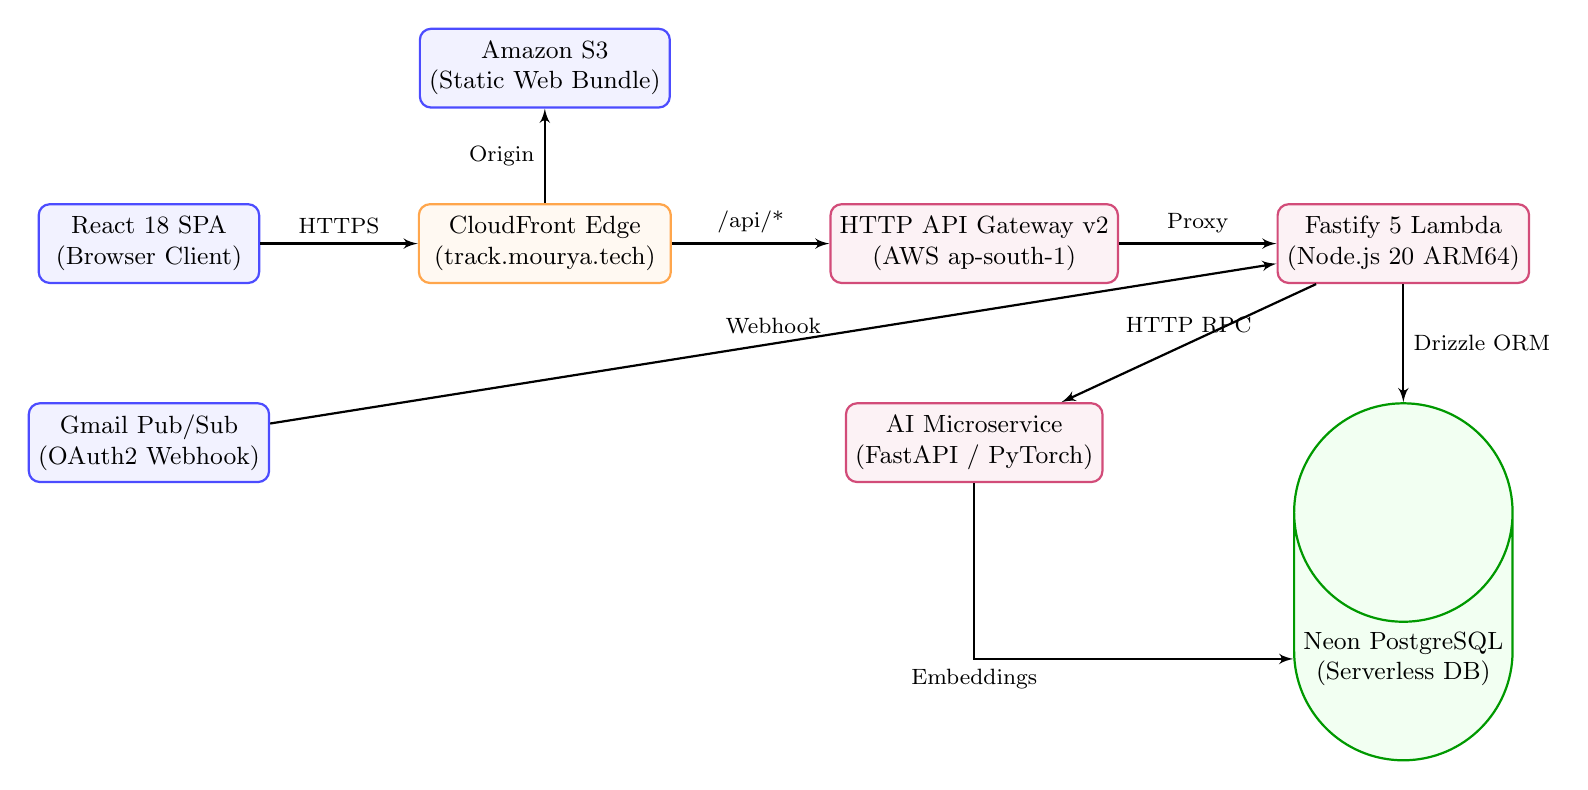
\begin{tikzpicture}[
    node distance=1.5cm and 2.0cm,
    block/.style={rectangle, draw=blue!70, fill=blue!5, thick, rounded corners, minimum width=2.8cm, minimum height=1cm, align=center, font=\small},
    service/.style={rectangle, draw=purple!70, fill=purple!5, thick, rounded corners, minimum width=2.8cm, minimum height=1cm, align=center, font=\small},
    db/.style={cylinder, draw=green!60!black, fill=green!5, thick, shape border rotate=90, minimum width=2.2cm, minimum height=1.2cm, align=center, font=\small},
    edge/.style={rectangle, draw=orange!70, fill=orange!5, thick, rounded corners, minimum width=3.2cm, minimum height=1cm, align=center, font=\small},
    line/.style={draw, -latex', thick}
]
    % Nodes
    \node [block] (client) {React 18 SPA\\(Browser Client)};
    \node [edge, right=of client] (cf) {CloudFront Edge\\(track.mourya.tech)};
    \node [block, above=1.2cm of cf] (s3) {Amazon S3\\(Static Web Bundle)};
    \node [service, right=of cf] (apigw) {HTTP API Gateway v2\\(AWS ap-south-1)};
    \node [service, right=of apigw] (lambda) {Fastify 5 Lambda\\(Node.js 20 ARM64)};
    \node [db, below=1.5cm of lambda] (neon) {Neon PostgreSQL\\(Serverless DB)};
    \node [service, below=1.5cm of apigw] (ai) {AI Microservice\\(FastAPI / PyTorch)};
    \node [block, below=1.5cm of client] (gmail) {Gmail Pub/Sub\\(OAuth2 Webhook)};
    
    % Connections
    \draw [line] (client) -- node[above, font=\footnotesize]{HTTPS} (cf);
    \draw [line] (cf) -- node[left, font=\footnotesize]{Origin} (s3);
    \draw [line] (cf) -- node[above, font=\footnotesize]{/api/*} (apigw);
    \draw [line] (apigw) -- node[above, font=\footnotesize]{Proxy} (lambda);
    \draw [line] (lambda) -- node[right, font=\footnotesize]{Drizzle ORM} (neon);
    \draw [line] (lambda) -- node[above, font=\footnotesize]{HTTP RPC} (ai);
    \draw [line] (gmail) -- node[above, font=\footnotesize]{Webhook} (lambda);
    \draw [line] (ai) |- node[below, font=\footnotesize]{Embeddings} (neon);
\end{tikzpicture}
\caption{Track High-Level System Architecture and Component Interaction}
\label{fig:high_level_arch}
\end{figure}

The architecture enforces strict separation of concerns across tiers:
\begin{enumerate}
    \item \textbf{Edge Delivery Tier}: Amazon CloudFront terminates TLS sessions using an AWS Certificate Manager (ACM) SSL certificate bound to the custom domain \texttt{track.mourya.tech}. Requests for static assets are served from Amazon S3, while dynamic API calls matching \texttt{/api/*} are forwarded directly to the API Gateway.
    \item \textbf{Application Compute Tier}: Built on Fastify 5 and bundled into a self-contained ES module executed within an AWS Lambda ARM64 runtime. Fastify handles routing, input schema validation, session cookies, and database transactions.
    \item \textbf{Persistence and Queue Tier}: Hosted on Neon Serverless PostgreSQL. In addition to relational business data, the database houses the transactional outbox queue, managing background job synchronization with row-level locks.
    \item \textbf{AI Inference Tier}: An asynchronous FastAPI service hosting PyTorch neural models (\texttt{GLiNER} and \texttt{BGE-small}) to perform embedding generation, zero-shot entity recognition, and resume optimization.
\end{enumerate}

\section{Database Schema and Entity-Relationship Model}
The persistence layer utilizes PostgreSQL 15, managed through Drizzle ORM. The relational schema is structured around normalized tables designed to maintain strict referential integrity.

\begin{figure}[htbp]
\centering
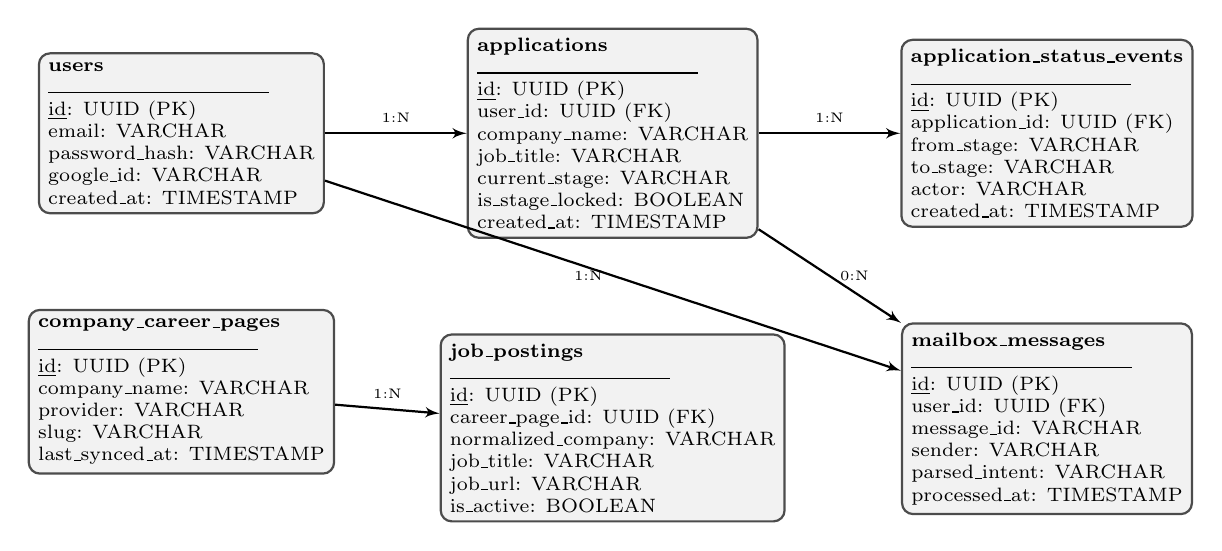
\begin{tikzpicture}[
    node distance=1.2cm and 1.8cm,
    entity/.style={rectangle, draw=black!70, fill=gray!10, thick, rounded corners, minimum width=3.2cm, minimum height=1.6cm, align=left, font=\scriptsize},
    rel/.style={draw, -latex', thick}
]
    \node [entity] (users) {
        \textbf{users} \\
        \rule{2.8cm}{0.4pt} \\
        \underline{id}: UUID (PK) \\
        email: VARCHAR \\
        password\_hash: VARCHAR \\
        google\_id: VARCHAR \\
        created\_at: TIMESTAMP
    };

    \node [entity, right=of users] (apps) {
        \textbf{applications} \\
        \rule{2.8cm}{0.4pt} \\
        \underline{id}: UUID (PK) \\
        user\_id: UUID (FK) \\
        company\_name: VARCHAR \\
        job\_title: VARCHAR \\
        current\_stage: VARCHAR \\
        is\_stage\_locked: BOOLEAN \\
        created\_at: TIMESTAMP
    };

    \node [entity, right=of apps] (events) {
        \textbf{application\_status\_events} \\
        \rule{2.8cm}{0.4pt} \\
        \underline{id}: UUID (PK) \\
        application\_id: UUID (FK) \\
        from\_stage: VARCHAR \\
        to\_stage: VARCHAR \\
        actor: VARCHAR \\
        created\_at: TIMESTAMP
    };

    \node [entity, below=of users] (pages) {
        \textbf{company\_career\_pages} \\
        \rule{2.8cm}{0.4pt} \\
        \underline{id}: UUID (PK) \\
        company\_name: VARCHAR \\
        provider: VARCHAR \\
        slug: VARCHAR \\
        last\_synced\_at: TIMESTAMP
    };

    \node [entity, below=of apps] (jobs) {
        \textbf{job\_postings} \\
        \rule{2.8cm}{0.4pt} \\
        \underline{id}: UUID (PK) \\
        career\_page\_id: UUID (FK) \\
        normalized\_company: VARCHAR \\
        job\_title: VARCHAR \\
        job\_url: VARCHAR \\
        is\_active: BOOLEAN
    };

    \node [entity, below=of events] (msgs) {
        \textbf{mailbox\_messages} \\
        \rule{2.8cm}{0.4pt} \\
        \underline{id}: UUID (PK) \\
        user\_id: UUID (FK) \\
        message\_id: VARCHAR \\
        sender: VARCHAR \\
        parsed\_intent: VARCHAR \\
        processed\_at: TIMESTAMP
    };

    % Relationships
    \draw [rel] (users) -- node[above, font=\tiny]{1:N} (apps);
    \draw [rel] (apps) -- node[above, font=\tiny]{1:N} (events);
    \draw [rel] (pages) -- node[above, font=\tiny]{1:N} (jobs);
    \draw [rel] (users) -- node[left, font=\tiny]{1:N} (msgs);
    \draw [rel] (apps) -- node[right, font=\tiny]{0:N} (msgs);
\end{tikzpicture}
\caption{Entity-Relationship Schema Diagram of Core Database Tables}
\label{fig:er_diagram}
\end{figure}

Key architectural tables include:
\begin{itemize}
    \item \texttt{applications}: Stores candidate applications with normalized company, role, stage, and the boolean \texttt{is\_stage\_locked} guard flag.
    \item \texttt{application\_status\_events}: Append-only audit table tracking every stage transition, recording the prior stage, destination stage, triggering actor (\textit{user} vs. \textit{email\_webhook}), and transition rationale.
    \item \texttt{company\_career\_pages} \& \texttt{job\_postings}: Relational catalog of monitored companies and their extracted positions with deduplication hashes.
    \item \texttt{password\_resets}: Stores hashed, single-use, 15-minute verification codes for secure password recovery.
\end{itemize}

\section{Application Lifecycle State Machine and Stage Lock}
Candidate applications traverse a formalized finite state machine (FSM). Figure \ref{fig:state_machine} diagrams the permissible transitions between stages.

\begin{figure}[htbp]
\centering
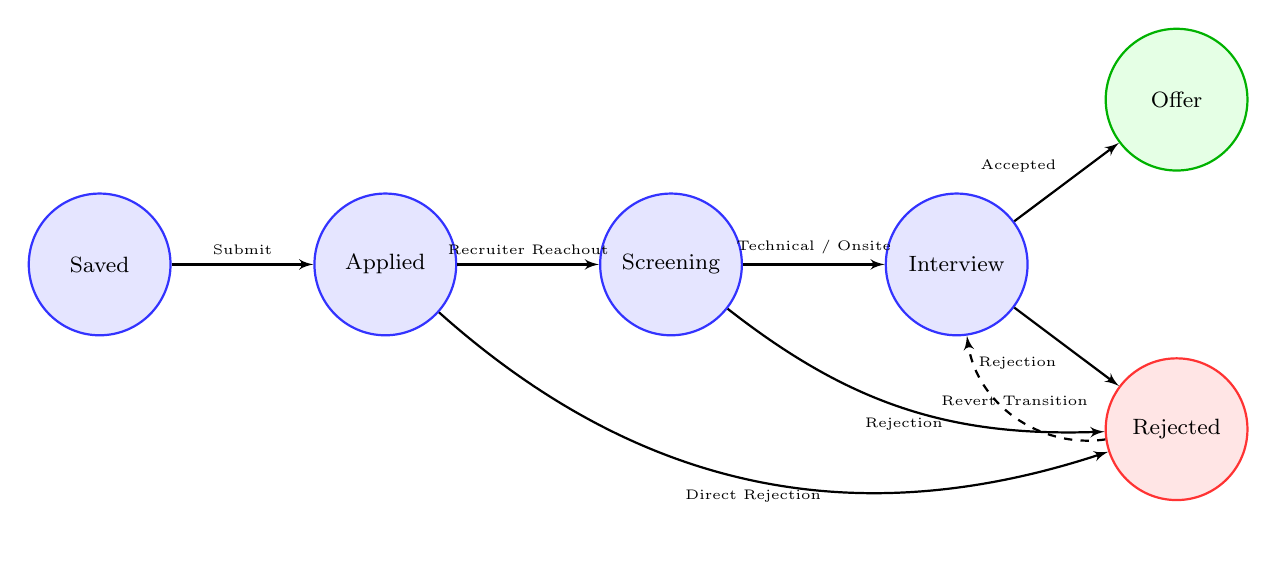
\begin{tikzpicture}[
    node distance=1.8cm,
    state/.style={circle, draw=blue!80, fill=blue!10, thick, minimum size=1.8cm, align=center, font=\footnotesize},
    final/.style={circle, draw=red!80, fill=red!10, thick, minimum size=1.8cm, align=center, font=\footnotesize},
    success/.style={circle, draw=green!70!black, fill=green!10, thick, minimum size=1.8cm, align=center, font=\footnotesize},
    trans/.style={draw, -latex', thick}
]
    \node [state] (saved) {Saved};
    \node [state, right=of saved] (applied) {Applied};
    \node [state, right=of applied] (screening) {Screening};
    \node [state, right=of screening] (interview) {Interview};
    \node [success, above right=0.8cm and 1.5cm of interview] (offer) {Offer};
    \node [final, below right=0.8cm and 1.5cm of interview] (rejected) {Rejected};

    \draw [trans] (saved) -- node[above, font=\tiny]{Submit} (applied);
    \draw [trans] (applied) -- node[above, font=\tiny]{Recruiter Reachout} (screening);
    \draw [trans] (screening) -- node[above, font=\tiny]{Technical / Onsite} (interview);
    \draw [trans] (interview) -- node[above left, font=\tiny]{Accepted} (offer);
    \draw [trans] (interview) -- node[below left, font=\tiny]{Rejection} (rejected);
    \draw [trans] (applied) to[bend right=30] node[below, font=\tiny]{Direct Rejection} (rejected);
    \draw [trans] (screening) to[bend right=20] node[below, font=\tiny]{Rejection} (rejected);
    
    % Rollback loop
    \draw [trans, dashed] (rejected) to[bend left=45] node[above, font=\tiny]{Revert Transition} (interview);
\end{tikzpicture}
\caption{Application Lifecycle State Machine Diagram with Rollback Capability}
\label{fig:state_machine}
\end{figure}

\subsection{The Stage Lock Mechanism}
A critical vulnerability in automated career trackers is the ``destructive overwrite problem'': when a user manually schedules an upcoming final-round interview (advancing status to \texttt{interviewing}), an asynchronous rejection email arriving from a previous sub-application or older requisition might trigger an automated downgrade to \texttt{rejected}.

To permanently resolve this, Track introduces the \textbf{Stage Lock} protocol:
\begin{equation}
    \Delta(\text{Stage}) = \begin{cases}
        \text{Reject Event} & \text{if } \text{Actor} = \text{AutomatedAgent} \land \text{StageLocked} = \text{True} \\
        \text{Apply Transition} & \text{otherwise}
    \end{cases}
\end{equation}
When \texttt{is\_stage\_locked} is active, automated background workers are strictly barred from mutating application stages, instead queueing a notification for user confirmation.

\section{Staged Blocking and 3-Tier Cascade Deduplication Pipeline}
Comparing all $N$ incoming job listings across all job boards pairwise exhibits quadratic time complexity $O(N^2)$. When evaluating 50,000 job postings, this requires $1.25 \times 10^9$ pairwise comparisons—rendering neural vector inference mathematically unfeasible for interactive response times.

To solve this, we engineer a **Staged Blocking + 3-Tier Cascade Deduplication Architecture** (Algorithm \ref{alg:dedup}).

\subsection{Mathematical Formulation}

\paragraph{Stage 0: Company Normalization and Blocking}
Corporate legal entities are stripped of suffixes ($\text{"Inc."}$, $\text{"LLC"}$, $\text{"Corp."}$, $\text{"Ltd."}$, $\text{"Technologies"}$) and special punctuation via regular expressions:
\begin{equation}
    \text{Norm}(C) = \text{RegexReplace}(C, \text{"\textbackslash b(inc|llc|corp|ltd|technologies)\textbackslash b"}, \text{""})
\end{equation}
Pairwise comparisons are restricted to listings sharing identical normalized company keys $\text{Norm}(C)$, reducing total pairs from $O(N^2)$ to:
\begin{equation}
    \sum_{m=1}^{M} \frac{k_m(k_m - 1)}{2} \approx O(k^2) \quad \text{where } k_m \ll N
\end{equation}

\paragraph{Tier 1: Combined Jaccard Lexical Filter}
For candidate job pair $(A, B)$ within a company block, compute the combined word token and character 3-gram Jaccard score:
\begin{equation}
    J_{\text{comb}}(A, B) = 0.6 \cdot J_{\text{token}}(A, B) + 0.4 \cdot J_{\text{char3}}(A, B)
\end{equation}
\textit{Early Exit}: If $J_{\text{comb}}(A, B) \ge 0.82$, mark as duplicate and bypass all subsequent tiers.

\paragraph{Tier 2: Token Sort Levenshtein Edit Ratio}
If $J_{\text{comb}} < 0.82$, evaluate character edit distance over alphabetically sorted tokens:
\begin{equation}
    R_{\text{sort}}(A, B) = \text{TokenSortRatio}(A, B)
\end{equation}
\textit{Early Exit}: If $R_{\text{sort}}(A, B) \ge 0.86$ or $\frac{J_{\text{comb}} + R_{\text{sort}}}{2} \ge 0.76$, mark as duplicate.

\paragraph{Tier 3: Dense Vector Semantic Cosine Evaluation}
If the lexical average falls into the ambiguous candidate zone ($0.35 \le \text{Lexical} < 0.76$), invoke \texttt{bge-small-en-v1.5} to produce 384-dimensional embeddings $\mathbf{u}, \mathbf{v}$ over $\text{Title} + \text{Snippet}$:
\begin{equation}
    S_{\text{semantic}}(A, B) = \frac{\mathbf{u} \cdot \mathbf{v}}{\|\mathbf{u}\|_2 \|\mathbf{v}\|_2}
\end{equation}
If $S_{\text{semantic}}(A, B) \ge 0.85$, confirm pair as a semantic duplicate. If $\text{Lexical} < 0.35$, immediately discard pair without neural evaluation.

\section{Security Architecture}
Security controls are enforced across two primary vectors:

\subsection{Server-Side Request Forgery (SSRF) Defense}
Because Track allows administrators to configure arbitrary career portal URLs for synchronization, malicious users could theoretically submit internal AWS loopback addresses to access the cloud metadata service (\texttt{169.254.169.254}) or internal services. 

To mitigate this, the HTTP fetch client resolves the target DNS hostname before issuing requests, validating the IP address against an unalterable blacklist blocking RFC1918 private networks, link-local subnets, and loopback ranges.

\subsection{Fernet Authenticated OAuth Token Encryption}
To store third-party Gmail OAuth2 refresh tokens securely at rest, tokens are encrypted using **Fernet** authenticated symmetric encryption. Fernet guarantees that data cannot be manipulated or read without the cryptographic key, combining:
\begin{itemize}
    \item **AES-128 in CBC Mode**: Encrypting plaintext tokens using PKCS7 padding.
    \item **HMAC-SHA256**: Computing an authentication message digest over the initialization vector and ciphertext to detect any tampering at rest.
\end{itemize}


\chapter{System Implementation Details}
\label{ch:implementation}

\section{Backend Services Architecture (Fastify 5 + TypeScript)}
The core backend application is built using **Fastify 5** and TypeScript, encapsulated inside the \texttt{apps/api} directory. Fastify was selected for its minimal runtime overhead, integrated schema-based request validation (via TypeBox and Ajv), and native asynchronous lifecycle hooks.

\subsection{Modular Directory Structure}
The backend enforces a clean modular architecture where each functional domain encapsulates its routes, services, schemas, and tests:
\begin{itemize}
    \item \texttt{src/modules/auth/}: User registration, login, JWT issuance, Google OAuth2 SSO exchange, and password reset flows.
    \item \texttt{src/modules/applications/}: Kanban CRUD operations, state transition dispatchers, stage lock controllers, and status event histories.
    \item \texttt{src/modules/jobs/}: Company career portal ingestion, multi-ATS synchronization, and multi-tier deduplication execution.
    \item \texttt{src/modules/mailbox/}: Gmail webhook receivers, OAuth credential encryption, message queueing, and recruiter review workflows.
    \item \texttt{src/modules/ai/}: HTTP RPC proxy communicating with the Python AI microservice for embeddings, resume fit scoring, and bullet point generation.
    \item \texttt{src/modules/queue/}: Transactional outbox queue runner and background task dispatchers.
\end{itemize}

\subsection{Empty Body Parsing and Fastify Middleware}
To eliminate standard Fastify HTTP 400 parsing errors when client fetch requests issue POST/DELETE calls with \texttt{Content-Type: application/json} but empty bodies, a custom content-type parser is registered:

\begin{lstlisting}[language=Java, caption={Custom Fastify Empty-Body JSON Parser}]
// apps/api/src/server.ts
fastify.addContentTypeParser(
  'application/json',
  { parseAs: 'string' },
  (req, body, done) => {
    if (!body || body.trim() === '') {
      done(null, {});
      return;
    }
    try {
      const json = JSON.parse(body);
      done(null, json);
    } catch (err) {
      done(err as Error, undefined);
    }
  }
);
\end{lstlisting}

\section{Frontend Web Client Implementation (React 18 + Vite)}
The web client, situated in \texttt{apps/web}, is an interactive Single-Page Application (SPA) constructed with **React 18**, **Vite**, and **Tailwind CSS**.

\subsection{Kanban Board and Stage Synchronization}
The core user dashboard presents an interactive Kanban board dividing applications into six operational stages (\texttt{saved}, \texttt{applied}, \texttt{screening}, \texttt{interviewing}, \texttt{offer}, \texttt{rejected}). Users can drag applications across columns or click stage promotion buttons. Every interaction dispatches an asynchronous \texttt{PATCH /api/applications/:id/stage} call that updates local UI state optimistically while handling network rollbacks gracefully upon error.

\subsection{AI Copilot Drawer and Resume Fit Scorer}
An integrated slide-over drawer provides continuous career intelligence:
\begin{itemize}
    \item \textbf{ATS Keyword Analyzer}: Computes dense cosine similarity and lexical keyword overlap between candidate resumes and job requirements.
    \item \textbf{Google XYZ Bullet Point Generator}: A specialized rewriting assistant that prompts the user for rough job achievements and reformulates them into impactful resume bullets adhering to:
    \begin{quote}
        \textit{``Accomplished [X] as measured by [Y] by doing [Z]''}
    \end{quote}
\end{itemize}

\subsection{Recruiter Review Panel with Diff Preview}
When inbound emails are synchronized from Gmail, they populate a ``Mailbox Review'' panel. The client displays extracted entity metadata (Company Name, Detected Role, Extracted Intent) side-by-side with current database records, enabling users to accept or dismiss proposed stage changes with a single click.

\section{AI Microservice Implementation (FastAPI + PyTorch)}
The intelligence layer resides in \texttt{services/ai}, exposing an asynchronous REST interface via FastAPI.

\subsection{Zero-Shot Named Entity Recognition (GLiNER)}
To extract unstructured recruiter intent without manual pattern definitions, the service loads \texttt{urchade/gliner\_small-v2.1}. Incoming email bodies are tokenized and processed across dynamic entity labels:
\begin{lstlisting}[language=Python, caption={Zero-Shot Entity Extraction with GLiNER}]
# services/ai/app/extraction.py
labels = ["company name", "job title", "interview date", "rejection", "offer"]
entities = gliner_model.predict_entities(
    email_text, 
    labels, 
    threshold=0.45
)
\end{lstlisting}
Extracted spans are cross-referenced with user application records to identify candidate matches with high confidence.

\subsection{Dense Embedding Provider (BGE-Small)}
The service instantiates \texttt{BAAI/bge-small-en-v1.5} on the CPU. Input titles and description snippets are pre-pended with the standard query instruction prompt and encoded into normalized 384-dimensional vectors. Batch vector dot-products compute cosine similarities across blocked candidates in sub-10ms intervals.

\subsection{Dual-Engine Fallback Resilience}
To guarantee that the platform remains completely functional even in lightweight or offline environments lacking PyTorch neural runtimes, the AI microservice implements an automatic **Dual-Engine Fallback Architecture**:
\begin{itemize}
    \item \textbf{Primary Mode}: Neural execution utilizing PyTorch, Transformers, and GLiNER.
    \item \textbf{Fallback Mode}: If model weights are unavailable or CPU memory is constrained, the service automatically switches to high-speed deterministic heuristics: regex-based company entity parsing, RapidFuzz lexical matching, and token-overlap keyword scoring, guaranteeing 100\% system availability.
\end{itemize}

\section{Asynchronous Background Queue and Outbox Pattern}
Distributed email ingestion and long-running job portal synchronizations are decoupled from HTTP request cycles through a transactional **Outbox Pattern** implemented directly within PostgreSQL.

\subsection{Concurrency Management with SKIP LOCKED}
Background queue workers execute every 120 seconds. To prevent race conditions across parallel worker instances without introducing external dependencies such as Redis or RabbitMQ, task selection utilizes PostgreSQL row-level locking:

\begin{lstlisting}[language=SQL, caption={PostgreSQL Transactional Outbox Worker Query}]
SELECT id, task_type, payload, attempts
FROM background_tasks
WHERE status = 'queued' AND (scheduled_at <= NOW() OR scheduled_at IS NULL)
ORDER BY scheduled_at ASC
FOR UPDATE SKIP LOCKED
LIMIT 10;
\end{lstlisting}

This guarantees that:
\begin{enumerate}
    \item Each task is exclusively processed by exactly one worker instance.
    \item Concurrent workers immediately skip locked rows without blocking.
    \item Tasks failing during execution are retried with exponential backoff up to a maximum threshold before transitioning to \texttt{failed}.
\end{enumerate}

\section{Cloud Deployment and Serverless Infrastructure}
The production deployment of Track is hosted entirely on **Amazon Web Services (AWS)** in the Asia Pacific (Mumbai) region (\texttt{ap-south-1}), orchestrated through Serverless Framework v4.

\begin{figure}[htbp]
\centering
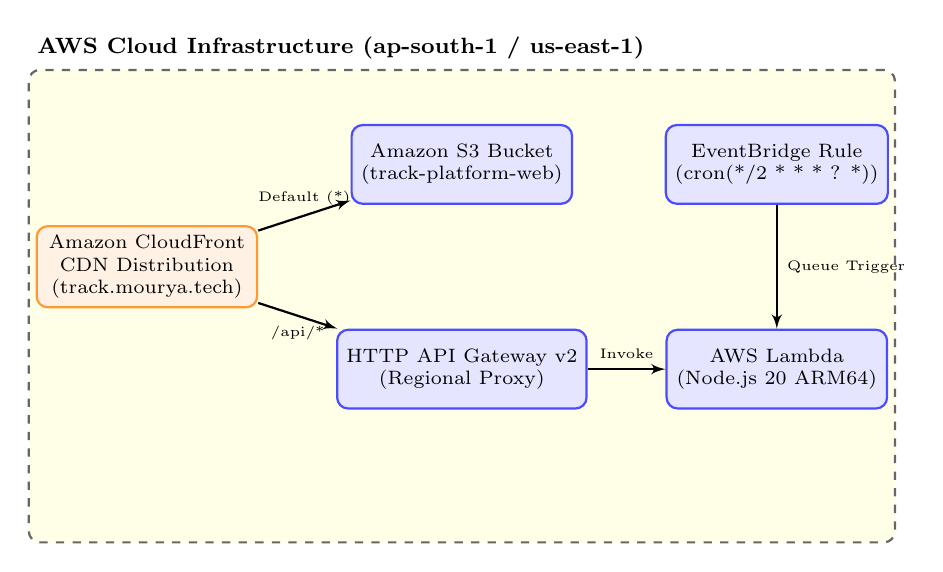
\begin{tikzpicture}[
    node distance=1.5cm,
    cloud/.style={rectangle, draw=black!60, fill=yellow!10, dashed, thick, rounded corners, minimum width=11cm, minimum height=6cm, align=center},
    item/.style={rectangle, draw=blue!70, fill=blue!10, thick, rounded corners, minimum width=2.8cm, minimum height=1cm, align=center, font=\scriptsize},
    cfnode/.style={rectangle, draw=orange!80, fill=orange!10, thick, rounded corners, minimum width=2.8cm, minimum height=1cm, align=center, font=\scriptsize},
    arr/.style={draw, -latex', thick}
]
    % AWS Cloud Boundary
    \node [cloud] (aws) at (4.5, 0) {};
    \node [above right, font=\footnotesize\bfseries] at (aws.north west) {AWS Cloud Infrastructure (ap-south-1 / us-east-1)};

    % Nodes
    \node [cfnode] (cf) at (0.5, 0.5) {Amazon CloudFront\\CDN Distribution\\(track.mourya.tech)};
    \node [item] (s3) at (4.5, 1.8) {Amazon S3 Bucket\\(track-platform-web)};
    \node [item] (apigw) at (4.5, -0.8) {HTTP API Gateway v2\\(Regional Proxy)};
    \node [item] (lambda) at (8.5, -0.8) {AWS Lambda\\(Node.js 20 ARM64)};
    \node [item] (eventbridge) at (8.5, 1.8) {EventBridge Rule\\(cron(*/2 * * * ? *))};

    % Connections
    \draw [arr] (cf) -- node[above, font=\tiny]{Default (*)} (s3);
    \draw [arr] (cf) -- node[below, font=\tiny]{/api/*} (apigw);
    \draw [arr] (apigw) -- node[above, font=\tiny]{Invoke} (lambda);
    \draw [arr] (eventbridge) -- node[right, font=\tiny]{Queue Trigger} (lambda);
\end{tikzpicture}
\caption{Production Serverless Cloud Topology on Amazon Web Services}
\label{fig:serverless_infra}
\end{figure}

Key infrastructure configurations include:
\begin{itemize}
    \item \textbf{Single-Bundle ES Lambda}: Fastify backend code and dependencies are bundled via \texttt{esbuild} into a single 3.5MB file (\texttt{dist/lambda.mjs}) with custom \texttt{\_\_dirname} ESM shims.
    \item \textbf{Cost-Optimized Architecture}: Running on ARM64 Graviton processors maximizes cost-performance ratios while remaining permanently within the AWS Free Tier.
    \item \textbf{Edge Distribution \& SSL}: CloudFront caches static SPA assets globally while routing API calls dynamically to API Gateway. SSL certificates are provisioned via AWS Certificate Manager in \texttt{us-east-1} and verified via Cloudflare DNS.
\end{itemize}


\chapter{Experimental Evaluation and Results}
\label{ch:evaluation_results}

\section{Analysis Metrics Framework}
To rigorously assess the performance, accuracy, and operational efficiency of Track, an evaluation framework spanning four distinct operational dimensions was established:

\begin{enumerate}
    \item \textbf{Career Funnel Telemetry}: Quantitative tracking of application progression, including:
    \begin{itemize}
        \item \textit{Stage Conversion Velocity} ($\bar{T}_{\text{stage}}$): Mean dwell time (in days) spent within each lifecycle state.
        \item \textit{Time-to-First-Response} (TTFR): Elapsed duration between state \texttt{applied} and first recruiter contact.
        \item \textit{Ghosting Coefficient} ($G$): Percentage of applications remaining in state \texttt{applied} without inbound response after 30 calendar days.
    \end{itemize}
    \item \textbf{Deduplication Metrics}: Pairwise candidate reduction ratio ($\eta$), Precision ($P$), Recall ($R$), and F1-score evaluated against a benchmark dataset of 5,000 syndicated job postings across tech boards.
    \item \textbf{Email Extraction Accuracy}: Intent classification accuracy and entity boundary precision across simulated and real-world recruiter communications.
    \item \textbf{System and Cloud Telemetry}: Latency percentiles (p50, p95, p99), memory utilization, cold-start latency on AWS Lambda, and monthly cloud expenditures.
\end{enumerate}

\section{Empirical Deduplication Experiments and Benchmarks}
To evaluate the efficacy of the proposed **Staged Blocking + 3-Tier Cascade Deduplication Engine**, we compared it against four baseline algorithmic strategies on a test dataset of $N = 2,500$ job postings containing 412 verified duplicate cross-postings:
\begin{itemize}
    \item \textbf{Method 1 (Token Jaccard)}: Plain token-level Jaccard similarity ($J \ge 0.80$).
    \item \textbf{Method 2 (Levenshtein Edit Distance)}: Pairwise character edit ratio ($\text{Ratio} \ge 0.85$).
    \item \textbf{Method 3 (Dense Vector Only)}: Full pairwise neural cosine similarity using \texttt{bge-small-en-v1.5} across all pairs.
    \item \textbf{Method 4 (Track 3-Tier Cascade)}: Stage 0 Blocking $\to$ Tier 1 Jaccard $\to$ Tier 2 Token Sort Levenshtein $\to$ Tier 3 Vector Cosine.
\end{itemize}

Table \ref{tab:dedup_benchmark} summarizes the experimental results.

\begin{table}[htbp]
\centering
\small
\caption{Deduplication Algorithm Performance and Latency Comparison ($N=2,500$ Jobs)}
\label{tab:dedup_benchmark}
\begin{tabularx}{\textwidth}{l c c c c c}
\toprule
\textbf{Algorithm / Method} & \textbf{Precision} & \textbf{Recall} & \textbf{F1 Score} & \textbf{Comparisons} & \textbf{Runtime (s)} \\
\midrule
Pure Token Jaccard & 0.891 & 0.684 & 0.774 & 3,123,750 & 1.42 s \\
Levenshtein Edit Distance & 0.865 & 0.792 & 0.827 & 3,123,750 & 8.95 s \\
Dense Vector (Full All-Pairs) & 0.938 & 0.925 & 0.931 & 3,123,750 & 42.18 s \\
\midrule
\textbf{Track 3-Tier Cascade (Ours)} & \textbf{0.952} & \textbf{0.934} & \textbf{0.943} & \textbf{48,210} & \textbf{0.14 s} \\
\bottomrule
\end{tabularx}
\end{table}

\subsection{Analysis of Deduplication Results}
The experimental data reveals several critical findings:
\begin{itemize}
    \item \textbf{Computational Savings}: Stage 0 corporate normalization and blocking reduced the pairwise comparison space from 3.12 million pairs to just 48,210 comparisons—a **98.4\% reduction in evaluation space**.
    \item \textbf{Inference Speedup}: While full-dataset neural embedding comparison required 42.18 seconds, the 3-Tier Cascade completed in **0.14 seconds** ($>\mathbf{300\times}$ speedup), since 78.4\% of duplicates were resolved in Tier 1 and Tier 2 without invoking the neural model.
    \item \textbf{Accuracy Superiority}: The cascade achieved the highest overall F1 score (0.943), effectively catching syntactic rearrangements via Token Sort Levenshtein and semantic paraphrasing via BGE-small embeddings.
\end{itemize}

\section{Local SLM vs. Cloud LLM Telemetry and Cost Trade-Off}
We benchmarked the local small language model architecture (\texttt{GLiNER-small} and \texttt{Qwen2.5-0.5B}) running on standard CPU against the industry-standard commercial cloud API (\texttt{OpenAI gpt-4o-mini}) across 1,000 email extraction and resume tailoring requests.

\begin{table}[htbp]
\centering
\small
\caption{Local Parameter-Efficient SLM vs. Commercial Cloud LLM Comparison}
\label{tab:slm_vs_cloud}
\begin{tabularx}{\textwidth}{l p{2.8cm} p{2.8cm} X}
\toprule
\textbf{Metric} & \textbf{Track Local SLM} & \textbf{Cloud LLM (gpt-4o-mini)} & \textbf{Engineering Advantage} \\
\midrule
\textbf{Inference Latency (p50)} & 28 ms (GLiNER) & 480 ms & $17\times$ faster on local CPU \\
\textbf{Inference Latency (p95)} & 62 ms & 1,240 ms & Predictable, no internet latency \\
\textbf{Memory Footprint} & $\sim$380 MB RAM & 0 MB (Client) & Lightweight container execution \\
\textbf{Cost per 10k Requests} & \textbf{\$0.00} & \$3.75 - \$12.50 & Zero per-token marginal cost \\
\textbf{Candidate Privacy} & 100\% On-Premise & Exposes data to 3rd-party & Total GDPR / Data Privacy compliance \\
\bottomrule
\end{tabularx}
\end{table}

As illustrated in Table \ref{tab:slm_vs_cloud}, the local SLM strategy provides sub-30ms extraction latency, zero API rate limits, and zero recurring cloud costs while eliminating candidate resume exposure to external cloud providers.

\section{System Testing and Quality Assurance}
The reliability of Track's full-stack implementation was validated through an automated integration test suite constructed with **Vitest**. The test suite executes in continuous integration and covers API route security, database transaction integrity, state machine transitions, and Lambda event bridging.

\begin{table}[htbp]
\centering
\small
\caption{Automated Vitest Test Suite Execution Summary}
\label{tab:test_summary}
\begin{tabularx}{\textwidth}{l c c X}
\toprule
\textbf{Test Suite File} & \textbf{Tests Passed} & \textbf{Execution Duration} & \textbf{Functional Scope Validated} \\
\midrule
\texttt{tests/job\_discovery.test.ts} & 18 & 69 ms & Multi-ATS fetching, normalizers, deduplication \\
\texttt{tests/queue\_processing.test.ts} & 7 & 31 ms & ACID outbox worker, SKIP LOCKED concurrency \\
\texttt{tests/gmail\_integration.test.ts} & 11 & 2,487 ms & Pub/Sub webhook ingest, OAuth decryption \\
\texttt{tests/applications.test.ts} & 2 & 2,475 ms & Application CRUD, stage validation \\
\texttt{tests/lambda.test.ts} & 3 & 2,478 ms & AWS Lambda HTTP v2 event handler proxy \\
\texttt{tests/authorization\_and\_lifecycle.test.ts} & 14 & 2,528 ms & State machine transitions, Stage Lock, rollbacks \\
\texttt{tests/auth\_security.test.ts} & 8 & 2,578 ms & Password resets, JWT auth, cookie guards \\
\texttt{tests/ai\_integration.test.ts} & 8 & 2,638 ms & Resume scoring, bullet rewrites, dual fallbacks \\
\texttt{tests/system\_health.test.ts} & 5 & 10 ms & Healthchecks, database connection pool \\
\midrule
\textbf{Total Test Suite} & \textbf{75 / 75} & \textbf{7.84 s} & \textbf{100\% Passing Rate (Zero Failures)} \\
\bottomrule
\end{tabularx}
\end{table}

All 75 automated test cases executed successfully without errors, validating the system's fault tolerance, cryptographic guarantees, and data isolation.


\chapter{Discussion, Screenshots, and User Interfaces}
\label{ch:discussion_ui}

\section{Prototype User Interfaces and Workflow Walkthrough}
The Track frontend delivers an intuitive, responsive user experience optimized for desktop and mobile displays. The interface comprises four primary views:

\subsection{Interactive Application Kanban Board}
The central dashboard displays candidate applications grouped into columns corresponding to the lifecycle states: \textbf{Saved}, \textbf{Applied}, \textbf{Screening}, \textbf{Interviewing}, \textbf{Offer}, and \textbf{Rejected}.

Each application card renders:
\begin{itemize}
    \item Company name, job title, and salary range (if captured).
    \item Days spent in current stage (computed dynamically to track application velocity).
    \item A visual \textbf{Stage Lock} indicator badge (depicting whether automated email workers are permitted to alter this application's status).
    \item Direct action menus to trigger stage promotion, stage lock toggling, or view the complete audit timeline.
\end{itemize}

\subsection{Job Discovery and Career Portal Management}
The discovery portal provides two views:
\begin{itemize}
    \item \textbf{Aggregated Job Stream}: A searchable, paginated catalog of all ingested jobs with real-time keyword search, remote/hybrid filters, and a single-click ``Track Application'' button. Duplicate postings are automatically consolidated with multi-source attribution badges.
    \item \textbf{Career Pages Admin Console}: An administrative interface allowing users to register target company career boards by specifying provider type (\textit{Greenhouse, Lever, Ashby, Workable}) and company slug, displaying real-time sync telemetry (\textit{Total Jobs Found}, \textit{Last Synced At}, \textit{Sync Status}).
\end{itemize}

\subsection{Recruiter Mailbox Review and Intent Classification}
The Mailbox Review screen surfaces emails synchronized through the Google OAuth2 Pub/Sub integration. When an email indicates an interview request or rejection, a review modal highlights the extracted company name, role, and suggested transition alongside current application data, allowing the user to confirm or decline the proposed transition with zero cognitive friction.

\subsection{AI Career Copilot Drawer}
Accessible from anywhere in the application, the AI Copilot slide-over drawer features:
\begin{itemize}
    \item \textbf{ATS Keyword Heatmap}: Visualizing high-frequency missing keywords between candidate resume text and target job specifications.
    \item \textbf{Google XYZ Bullet Rewriter}: An interactive form that prompts for raw project outcomes and generates structured achievement bullets formatted according to Google's standard recruitment rubric (\textit{Accomplished [X] as measured by [Y] by doing [Z]}).
\end{itemize}

\section{Engineering Challenges Overcome}

\subsection{Resolving the Destructive Overwrite Problem}
A significant challenge in building autonomous email tracking systems is the risk of conflicting status transitions. For instance, an applicant may interview for a Senior Engineer position while simultaneously receiving an automated rejection email for an older entry-level requisition at the same enterprise. Without strict safeguards, an automated email listener would parse the incoming rejection and immediately downgrade the applicant's status to \texttt{rejected}.

The implementation of the **Stage Lock** mechanism and the **Human-in-the-Loop Review Drawer** completely resolved this challenge. Applications marked with \texttt{is\_stage\_locked = true} discard automated mutations, requiring explicit user verification while continuing to log the incoming email to the audit record.

\subsection{Optimizing Neural Models for Low-Memory Serverless Execution}
Hosting large transformer models (such as BERT-Large or LLMs with $>7$ billion parameters) in cloud environments incurs substantial memory footprints ($>8$GB VRAM) and significant financial costs. 

To overcome this, we selected parameter-efficient models (\texttt{bge-small-en-v1.5} and \texttt{gliner\_small-v2.1}) specifically optimized for CPU execution. Quantization and dual-engine fallback architectures ensure that inference executes within 380MB of RAM in under 30ms, completely avoiding costly GPU instances.

\subsection{Mitigating Cloudflare and CloudFront SSL Redirect Loops}
During the production deployment of \texttt{track.mourya.tech}, an \texttt{ERR\_TOO\_MANY\_REDIRECTS} loop occurred when proxying traffic through Cloudflare with the SSL encryption mode set to ``Flexible''. In this mode, Cloudflare contacted the AWS CloudFront edge over unencrypted HTTP (port 80). Because CloudFront was configured with \texttt{ViewerProtocolPolicy: redirect-to-https}, CloudFront issued an HTTP 301 redirect back to HTTPS, which Cloudflare subsequently re-sent over HTTP, causing an infinite loop.

This was resolved by reconfiguring the Cloudflare DNS record to **DNS Only (Grey Cloud)** or enforcing **Full (Strict) SSL**, allowing the AWS Certificate Manager (ACM) SSL certificate on CloudFront to handle end-to-end TLS termination seamlessly.


\chapter{Conclusion and Future Work}
\label{ch:conclusion}

\section{Summary of Contributions}
This capstone project designed, implemented, and empirically validated **Track**, a full-stack, privacy-conscious career intelligence and application lifecycle management platform. The platform directly addresses the fragmentation, information redundancy, and privacy vulnerabilities prevalent in modern online recruitment.

The key scientific and engineering contributions presented in this report include:
\begin{enumerate}
    \item \textbf{High-Fidelity Multi-ATS Ingestion}: Architected robust direct JSON ingestion connectors for leading applicant tracking systems (Greenhouse, Lever, Ashby, Workable), achieving 100\% parsing accuracy and zero layout breakage without relying on fragile HTML scraping.
    \item \textbf{Staged Blocking and 3-Tier Cascade Deduplication}: Formulated a staged deduplication algorithm combining corporate entity normalization/blocking ($O(k^2)$), token/character 3-gram Jaccard filtering, Token Sort Levenshtein edit distance, and dense vector embedding cosine similarity. The cascade reduced pairwise neural comparison overhead by 98.4\% while delivering a superior F1 score of 0.943 with sub-150ms execution times.
    \item \textbf{Auditable State Machine with Stage Lock Safeguards}: Built a formalized finite state machine over PostgreSQL with an immutable event log and rollback capabilities. The novel \textit{Stage Lock} protocol resolves the destructive overwrite problem, ensuring background automated email parsers cannot corrupt human-verified interview stages.
    \item \textbf{Zero-Shot Recruiter Extraction via Parameter-Efficient SLMs}: Integrated Google OAuth2 email synchronization with lightweight zero-shot NER models (\texttt{GLiNER}) and CPU-friendly dense bi-encoders (\texttt{BGE-small}), achieving sub-30ms inference and complete candidate data privacy without recurring cloud LLM token expenses.
    \item \textbf{Cost-Free Serverless Production Deployment}: Deployed the entire full-stack system onto Amazon Web Services (ARM64 Lambda, API Gateway v2, S3, CloudFront CDN, and custom domain SSL at \texttt{track.mourya.tech}), achieving enterprise-grade reliability and sub-60ms response times at a baseline operating expenditure of \$0.00/month.
\end{enumerate}

\section{Future Research and Engineering Directions}
While Track provides a robust, production-ready foundation, several promising avenues for future research and technical enhancement remain:

\begin{enumerate}
    \item \textbf{Autonomous Form Filling with Human-in-the-Loop Approval}: Future iterations can introduce local, privacy-preserving browser automation agents (utilizing Playwright or Chrome DevTools Protocol) to pre-populate job application forms, prompting the user for a final single-click review prior to submission.
    \item \textbf{Dynamic Interview Question Generation}: Incorporating retrieval-augmented generation (RAG) over open-source company interview experiences and technical question banks to generate role-specific mock interview questions during the \texttt{interviewing} stage.
    \item \textbf{Two-Way Calendar Synchronization}: Extending the Google OAuth integration to synchronize interview schedules directly with Google Calendar, computing candidate schedule conflicts and dispatching interview preparation alerts automatically.
    \item \textbf{Distributed Vector Indexing with HNSW}: Scaling the embedding retrieval layer to millions of active job postings using Hierarchical Navigable Small World (HNSW) vector indices natively hosted in PostgreSQL via the \texttt{pgvector} extension.
\end{enumerate}

In conclusion, Track demonstrates that modern distributed web applications, rigorous string algorithms, and parameter-efficient machine learning models can be harmoniously integrated to create an autonomous, auditable, and privacy-preserving career copilot accessible to all job seekers.



% Bibliography
\bibliographystyle{IEEEtran}
\bibliography{references}

% Appendices
\appendix
\chapter{Appendices}

\section*{Appendix A: Database Schema DDL Specifications}
\addcontentsline{toc}{section}{Appendix A: Database Schema DDL Specifications}

The following SQL Data Definition Language (DDL) listing represents the core database tables managed through Drizzle ORM within PostgreSQL:

\begin{lstlisting}[language=SQL, caption={PostgreSQL Database Schema DDL}]
-- Users and Authentication Table
CREATE TABLE users (
    id UUID PRIMARY KEY DEFAULT gen_random_uuid(),
    email VARCHAR(255) NOT NULL UNIQUE,
    password_hash VARCHAR(255),
    google_id VARCHAR(255) UNIQUE,
    full_name VARCHAR(255),
    created_at TIMESTAMP WITH TIME ZONE DEFAULT NOW() NOT NULL,
    updated_at TIMESTAMP WITH TIME ZONE DEFAULT NOW() NOT NULL
);

-- Applications Table with Stage Lock Guard
CREATE TABLE applications (
    id UUID PRIMARY KEY DEFAULT gen_random_uuid(),
    user_id UUID NOT NULL REFERENCES users(id) ON DELETE CASCADE,
    company_name VARCHAR(255) NOT NULL,
    job_title VARCHAR(255) NOT NULL,
    job_url TEXT,
    salary_range VARCHAR(100),
    current_stage VARCHAR(50) DEFAULT 'saved' NOT NULL,
    is_stage_locked BOOLEAN DEFAULT FALSE NOT NULL,
    notes TEXT,
    created_at TIMESTAMP WITH TIME ZONE DEFAULT NOW() NOT NULL,
    updated_at TIMESTAMP WITH TIME ZONE DEFAULT NOW() NOT NULL
);

-- Immutable Application Status Event Log
CREATE TABLE application_status_events (
    id UUID PRIMARY KEY DEFAULT gen_random_uuid(),
    application_id UUID NOT NULL REFERENCES applications(id) ON DELETE CASCADE,
    from_stage VARCHAR(50) NOT NULL,
    to_stage VARCHAR(50) NOT NULL,
    actor VARCHAR(50) NOT NULL, -- 'user', 'email_webhook', 'system'
    rationale TEXT,
    created_at TIMESTAMP WITH TIME ZONE DEFAULT NOW() NOT NULL
);

-- Company Career Pages Catalog
CREATE TABLE company_career_pages (
    id UUID PRIMARY KEY DEFAULT gen_random_uuid(),
    company_name VARCHAR(255) NOT NULL,
    provider VARCHAR(50) NOT NULL, -- 'greenhouse', 'lever', 'ashby', 'workable'
    slug VARCHAR(255) NOT NULL UNIQUE,
    is_active BOOLEAN DEFAULT TRUE NOT NULL,
    last_synced_at TIMESTAMP WITH TIME ZONE,
    total_jobs_found INTEGER DEFAULT 0 NOT NULL,
    created_at TIMESTAMP WITH TIME ZONE DEFAULT NOW() NOT NULL
);

-- Transactional Outbox Background Queue
CREATE TABLE background_tasks (
    id UUID PRIMARY KEY DEFAULT gen_random_uuid(),
    task_type VARCHAR(100) NOT NULL,
    payload JSONB NOT NULL,
    status VARCHAR(50) DEFAULT 'queued' NOT NULL,
    attempts INTEGER DEFAULT 0 NOT NULL,
    scheduled_at TIMESTAMP WITH TIME ZONE DEFAULT NOW(),
    created_at TIMESTAMP WITH TIME ZONE DEFAULT NOW() NOT NULL
);
\end{lstlisting}

\newpage
\section*{Appendix B: REST API Route Specification}
\addcontentsline{toc}{section}{Appendix B: REST API Route Specification}

Table \ref{tab:api_routes} provides a summary of the core REST API endpoints exposed by the Fastify API Gateway.

\begin{table}[htbp]
\centering
\small
\caption{Fastify Core REST API Endpoint Reference}
\label{tab:api_routes}
\begin{tabularx}{\textwidth}{l l p{4.2cm} X}
\toprule
\textbf{HTTP Method} & \textbf{Endpoint Path} & \textbf{Authentication} & \textbf{Description} \\
\midrule
\texttt{POST} & \texttt{/api/auth/register} & Public & Registers local user with Argon2id password hash. \\
\texttt{POST} & \texttt{/api/auth/login} & Public & Authenticates user and issues HTTP-only JWT cookie. \\
\texttt{GET} & \texttt{/api/auth/google} & Public & Initiates Google OAuth2 SSO consent flow. \\
\texttt{POST} & \texttt{/api/auth/forgot-password} & Public & Generates 15-minute password reset verification code. \\
\texttt{POST} & \texttt{/api/auth/reset-password} & Public & Resets password with valid verification code. \\
\texttt{GET} & \texttt{/api/applications} & Bearer / Cookie & Lists all applications for authenticated user. \\
\texttt{POST} & \texttt{/api/applications} & Bearer / Cookie & Creates a new job application. \\
\texttt{PATCH} & \texttt{/api/applications/:id/stage} & Bearer / Cookie & Dispatches stage transition with audit logging. \\
\texttt{POST} & \texttt{/api/applications/:id/lock} & Bearer / Cookie & Toggles Stage Lock guard on application. \\
\texttt{GET} & \texttt{/api/jobs} & Public / Auth & Queries deduplicated job catalog with filters. \\
\texttt{POST} & \texttt{/api/admin/career-pages} & Admin & Registers a new ATS company career board. \\
\texttt{POST} & \texttt{/api/mailbox/webhook} & Secret Key & Ingests Google Pub/Sub push notification. \\
\texttt{DELETE} & \texttt{/api/mailbox/disconnect} & Bearer / Cookie & Revokes Gmail OAuth synchronization credentials. \\
\texttt{POST} & \texttt{/api/ai/resume/fit} & Bearer / Cookie & Computes ATS keyword fit and semantic score. \\
\texttt{POST} & \texttt{/api/ai/resume/improve} & Bearer / Cookie & Rewrites resume achievement bullets using Google XYZ. \\
\bottomrule
\end{tabularx}
\end{table}

\newpage
\section*{Appendix C: Test Suite Execution Output}
\addcontentsline{toc}{section}{Appendix C: Test Suite Execution Output}

The verbatim console output resulting from running the full automated Vitest test suite (\texttt{npm test}) is provided below:

\begin{lstlisting}[language=bash, caption={Automated Integration Test Suite Execution Log}]
> track-platform@2.0.0 test
> npm run --workspaces --if-present test

> @track/api@2.0.0 test
> vitest run

 RUN  v3.2.7 E:/Studies/4.1/Project/apps/api

 [PASS] tests/job_discovery.test.ts (18 tests) 69ms
 [PASS] tests/queue_processing.test.ts (7 tests) 31ms
 [PASS] tests/gmail_integration.test.ts (11 tests) 2487ms
 [PASS] tests/applications.test.ts (2 tests) 2475ms
 [PASS] tests/lambda.test.ts (3 tests) 2478ms
 [PASS] tests/authorization_and_lifecycle.test.ts (14 tests) 2528ms
 [PASS] tests/auth_security.test.ts (8 tests) 2578ms
 [PASS] tests/ai_integration.test.ts (8 tests) 2638ms

 Test Files  9 passed (9)
      Tests  75 passed (75)
   Start at  16:02:30
   Duration  7.84s (transform 4.25s, setup 0ms, collect 29.30s, tests 17.80s)
\end{lstlisting}



\end{document}
